% Notes:
% - The point that central regions of low J_z, density flattens = no constraining power
% - The condition on d(r_z)/d(r_z')
% - Widmark papers
% - https://arxiv.org/abs/2303.18040


% Reframe paper:
% - "Direct contouring" has advantage that don't have to assume Phi(x) or rho(x)
% - Disadvantage that physics doesn't have to be obeyed - contours can imply Phi that depends on v_z
% - Also: Under assumption of orbits, can compute actions angles freqs

% \begin{figure}[!t]
% \begin{center}
% % \includegraphics[width=0.9\textwidth]{visitstats.pdf}
% {\color{red} Figure placeholder}
% \end{center}
% \caption{%
% TODO
% \label{fig:chiplots}
% }
% \end{figure}

\PassOptionsToPackage{usenames,dvipsnames}{xcolor}
\documentclass[modern]{aastex631}
% \documentclass[twocolumn]{aastex631}

% Load common packages
\usepackage{microtype}  % ALWAYS!
\usepackage{amsmath}
\usepackage{amsfonts}
\usepackage{amssymb}
\usepackage{booktabs}
\usepackage{graphicx}
% \usepackage{color}

\usepackage{enumitem}
\setlist[description]{style=unboxed}

% Some style hacks:
\renewcommand{\twocolumngrid}{\onecolumngrid}
\setlength{\parindent}{1.1\baselineskip}
\addtolength{\topmargin}{-0.2in}
\addtolength{\textheight}{0.4in}
\sloppy\sloppypar\raggedbottom\frenchspacing

\graphicspath{{figures/}}
% \definecolor{cbblue}{HTML}{3182bd}
% \usepackage{hyperref}
% \definecolor{linkcolor}{rgb}{0.02,0.35,0.55}
% \definecolor{citecolor}{rgb}{0.45,0.45,0.45}
% \hypersetup{colorlinks=true,linkcolor=linkcolor,citecolor=citecolor,
%             filecolor=linkcolor,urlcolor=linkcolor}
% \hypersetup{pageanchor=true}

\newcommand{\documentname}{\textsl{Article}}
\newcommand{\sectionname}{Section}
\renewcommand{\figurename}{Figure}
\newcommand{\equationname}{Equation}
\renewcommand{\tablename}{Table}

% Missions
\newcommand{\project}[1]{\textsl{#1}}

% Packages / projects / programming
\newcommand{\package}[1]{\textsl{#1}}
\newcommand{\acronym}[1]{{\small{#1}}}
\newcommand{\github}{\package{GitHub}}
\newcommand{\python}{\package{Python}}
\newcommand{\jax}{\package{JAX}}
\newcommand{\emcee}{\project{emcee}}

% Stats / probability
\newcommand{\given}{\,|\,}
\newcommand{\norm}{\mathcal{N}}
\newcommand{\pdf}{\textsl{pdf}}

% Maths
\newcommand{\dd}{\mathrm{d}}
\newcommand{\deriv}[2]{\frac{\mathrm{d}{#1}}{\mathrm{d}{#2}}}
\newcommand{\dderiv}[2]{\frac{\mathrm{d^2}{#1}}{\mathrm{d}{#2}^2}}
\newcommand{\Deriv}[2]{\frac{\mathrm{D}{#1}}{\mathrm{D}{#2}}}
\newcommand{\pderiv}[2]{\frac{\partial {#1}}{\partial {#2}}}
\newcommand{\ppderiv}[2]{\frac{\partial^2 {#1}}{\partial {#2}^2}}
\newcommand{\transpose}[1]{{#1}^{\mathsf{T}}}
\newcommand{\inverse}[1]{{#1}^{-1}}
\newcommand{\argmin}{\operatornamewithlimits{argmin}}
\newcommand{\mean}[1]{\left< #1 \right>}

% Non-scalar variables
\renewcommand{\vec}[1]{\ensuremath{\bs{#1}}}
\newcommand{\mat}[1]{\ensuremath{\mathbf{#1}}}

% Units:
% Workaround for siunitx + AASTeX
% https://tex.stackexchange.com/questions/192610/use-emulateapj-aastex-with-siunitx
\usepackage{savesym}
\savesymbol{tablenum}
\usepackage{siunitx}
\restoresymbol{SIX}{tablenum}
\DeclareSIUnit\year{yr}
\DeclareSIUnit\parsec{pc}
\DeclareSIUnit\Msun{M_\odot}
\DeclareSIUnit\Rsun{R_\odot}
\newcommand{\mas}{\unit{\milli\arcsecond}}
\newcommand{\muas}{\unit{\micro\arcsecond}}
\newcommand{\kms}{\unit{\km\per\s}}
\newcommand{\kpc}{\unit{\kilo\parsec}}



% Misc.
\newcommand{\bs}[1]{\boldsymbol{#1}}

% Astronomy
\newcommand{\DM}{{\rm DM}}
\newcommand{\feh}{\ensuremath{{[{\rm Fe}/{\rm H}]}}}
\newcommand{\mh}{\ensuremath{{[{\rm M}/{\rm H}]}}}
\newcommand{\logg}{\ensuremath{\log g}}
\newcommand{\Teff}{\ensuremath{T_{\textrm{eff}}}}
\newcommand{\vsini}{\ensuremath{v\,\sin i}}
\newcommand{\mtwomin}{\ensuremath{M_{2, {\rm min}}}}

% Dynamics
\newcommand{\df}{\acronym{DF}}

% TO DO
\newcommand{\todo}[1]{{\color{red} TODO: #1}}
\newcommand{\placeholder}[1]{{\color{purple} #1}}

\newcommand{\gaia}{\textsl{Gaia}}
\newcommand{\dr}[1]{\acronym{DR}#1}
\newcommand{\apogee}{\acronym{APOGEE}}
\newcommand{\sdss}{\acronym{SDSS}}
\newcommand{\sdssiv}{\acronym{SDSS-IV}}
\newcommand{\thejoker}{\project{The~Joker}}


\shorttitle{}
\shortauthors{Price-Whelan et al.}

\begin{document}

\title{
    Data-driven Dynamics with Orbital Torus Imaging:  \\
    A Flexible Model of the Vertical Phase-space of the Galaxy
}
% ChatGPT: Empirical Modeling of Vertical Phase-Space Density in the Milky Way: A Flexible Method for Inferring the Acceleration Field

\newcommand{\affcca}{
    Center for Computational Astrophysics, Flatiron Institute, \\
    162 Fifth Ave, New York, NY 10010, USA
}

\author[0000-0003-0872-7098]{Adrian~M.~Price-Whelan}
\affiliation{\affcca}
\email{aprice-whelan@flatironinstitute.org}
\correspondingauthor{Adrian M. Price-Whelan}

\author{Jason~A.~S.~Hunt}
\affiliation{\affcca}

\author{Daniel~Horta~Darrington}
\affiliation{\affcca}

\author{Kathryn Johnston}
% \affiliation{\affcolumbia}

% TODO: orcid, affs
\author{David~W.~Hogg}
% \affiliation{\affcca}
% \affiliation{\affnyu}
% \affiliation{\affmpia}

\author{Lawrence Widrow}

\author{Benjamin~Cassese}

\author{Neige Frankel}

\author{+ more, ORDER TBD!}


\begin{abstract}\noindent
\emph{Old abstract - needs rethinking}
% Context
In a steady-state dynamical system, spatial gradients of the phase-space density (the
distribution function, \df) of any tracers are related to gradients of the underlying
gravitational potential (the acceleration field).
This is the basis of many methods used in Galactic dynamics to infer the mass or dark
matter distribution of the Milky Way, often with highly-symmetric, few-component,
parametric models of the Galaxy (e.g., an exponential disk with constant scale height).
However, we know that the Galaxy is not in equilibrium and its mass distribution is
complex:
Stellar kinematics show signatures of non-steady-state dynamics throughout the Galactic
disk and significant departures from axisymmetry.
% Aims
We aim to develop a framework for measuring the acceleration field of the Milky Way, in
the presence of weak disequilibrium, that makes few assumptions about the form of the
mass distribution.
% Methods
Here we outline a flexible method for empirically modeling the vertical phase-space
density (or mean statistics of stellar invariants in this phase-space, like element
abundances) of stars in the Galactic disk.
This method --- an improved version of the method of \emph{Orbital Torus Imaging} (OTI)
--- works by exploiting the fact that orbital trajectories in the vertical phase-space
of an unperturbed galaxy have predictable symmetries in projections of phase-space and
can be represented as a low-order Fourier expansion away from an ellipse.
% Results
We first demonstrate OTI using a toy simulation of a vertical phase-space distribution
of stars, then with a more realistic galactic disk population, and show that in both
cases OTI recovers the local vertical acceleration as a function of height above the
galactic midplane.
We then show that this method enables us to compute \emph{empirical} orbital actions,
angles, and frequencies for stars where the approximation of a separable 1D phase-space
is valid: This enables interpreting the timescales of disequilibrium features in a
flexible way that does not require adopting a global model of the gravitational
potential.
For example, we demonstrate that this method provides a useful tool for studying the
\emph{residuals} away from an equilibrium model, such as the ``\gaia\ Phase Spiral.''
% Conclusions
Some conclusions.

% Context
% Orbital dynamics is complex in six-dimensional phase-space, making it a challenge to
% interpret the rich and structured kinematic data of stars in the Milky Way revealed in
% recent data releases from the \gaia\ Mission.
% In a symmetric, steady-state galaxy, or in the presence of only weak perturbations, the
% dynamical interpretation and investigation of kinematic data is often simplified by
% using dynamical invariants such as orbital actions.
% However, computing many such quantities (e.g., the energy, actions, fundamental
% frequencies, etc.) require having a model for the gravitational potential and, even so,
% are either slow to compute or imprecise.
% % Aims
% To mitigate at least one of these limitations, we aim to demonstrate a method for
% estimating fundamental galactic orbital properties for stars directly from the kinematic
% and stellar label data (e.g., element abundances) without requiring a gravitational
% potential model.
% % Methods
% This method still assumes a symmetric and steady-state distribution function, but uses
% either the number density of stars in a slice of phase-space (e.g., vertical $z$--$v_z$
% kinematics) or a statistic computed from other stellar invariants in this slice (e.g.,
% element abundances) to empirically estimate orbital actions, frequencies, and angles for
% the stars.
% % Results
% We demonstrate the method using a toy equilibrium model where orbital properties are
% known, and then show applications of this method even in the presence of disequilibrium.
% As a last demonstration, we use data from the \gaia\ Mission to estimate the total mass
% density at the Galactic midplane as a function of radius near the sun.
% % Conclusions
% We conclude :shrugs:.

\end{abstract}

% \keywords{}

\section{Introduction} \label{sec:intro}

Measuring and studying the mass distribution of the Milky Way is an important venture
for many applications in astrophysics.
For one, the total mass distribution determines the orbits of its gas, stars, star
clusters, and satellite galaxies, and thus enables interpreting the kinematic snapshot
we observe in terms of dynamical and galactic evolutionary processes.
The Galactic mass distribution also encodes the structure of dark matter around the
Milky Way, which provides an important laboratory for studying the astrophysical
properties of dark matter on the scale of an individual galaxy.
On these mass scales (and smaller), effective models for dark matter predict different
density profiles and different populations of substructures.
We therefore hope that precise measurements of the structure of dark matter within the
Milky Way and other nearby galaxies will enable new constraints on the particle nature
of dark matter.

Until direct measurements of the Galactic acceleration field become more ubiquitous
(CITE), our best hope for studying the mass and dark matter content of the Milky Way
comes from modeling stellar kinematics (CITE binney tremaine).
The principle challenge of this problem is that we only observe a \emph{snapshot} of the
kinematics (i.e. position $\bs{x}$ and velocity $\bs{v}$) and other stellar properties
(i.e. element abundance, age, etc.) of stars throughout the Galaxy at present day.
That is, we do not observe the orbits of stars or even segments of their orbits, which
would enable a more direct measurement of the acceleration field around those
orbits.\footnote{TODO: note about phase coherence - conceptually, streams show us
orbits.}
Instead, we have to rely on statistical mechanics to relate the snapshot of tracer
kinematics we observe to the underlying mass distribution (CITE intro of Kuijken \&
Gilmore).

The fundamental objects of a statistical approach to Galactic dynamics are the tracer
distribution function (DF), $f(\bs{x}, \bs{v}, t)$, which describes the probability of
observing a star at position $\bs{x}$ and velocity $\bs{v}$ at time $t$, and the total
gravitational potential, $\Phi(\bs{x}, t)$, which is related to the mass density
distribution we seek $\rho(\bs{x}, t)$ through Poisson's equation $\nabla^2 \Phi = 4\pi
G \, \rho$.
Many dynamical inference methods have been built to connect these two objects (the DF
and the potential) in order to measure properties of the mass distribution of the Milky
Way and other galaxies (CITE).
These methods can be broadly categorized into two classes: those that work with
gradients of the DF to measure gradients of the potential (CITE), or those that model
the form of the DF itself (CITE).
In either case, the majority of applications of these methods have assumed that the
Galaxy is in equilibrium and the DF is in steady state so that the explicit time
dependence of the DF and potential can be ignored.
Most applications also assume that the DF and potential are separable in some
coordinates (for example, cylindrical radius $R$ and height $z$, for disk modeling), and
that the DF and/or potential can be expressed by a set of smooth, parametric model terms
for which the parameters can be inferred from the data.
These methods and assumptions have enabled a wide array of measurements of the structure
and mass distribution of the Milky Way's disk, central region, stellar halo, and dark
matter content over the last century (CITE).

Contemporary stellar surveys have opened up a new era of Galactic dynamical inferences
by providing an abundance of high-quality stellar label and kinematic data for millions
to billions of stars throughout our Galaxy.
This includes the transformative astrometric, photometric, and spectroscopic data from
the \gaia\ Mission (CITE), deep, multi-band photometric surveys such as the Sloan
Digital Sky Survey (SDSS; CITE), and high-resolution spectroscopic surveys such as the
Apache Point Observatory Galactic Evolution Experiment (APOGEE; CITE).
Many other stellar surveys are currently underway or planned for the near future that
will expand (or are expanding) the volume, number of stars, and precision of the
available data for Milky Way stars even further (CITE; LAMOST, GALAH, WEAVE, 4MOST,
SDSS-V).

The wealth of stellar survey data presently available brings an opportunity to make
precise measurements of the detailed structure of dark matter throughout the Milky Way
and learn about its formation history (CITE).
However, the current data volume and precision presents a challenge to current and past
dynamical inference methods that make use of stellar kinematics.
Many of these methods rely on assumptions that are violated at very high signal-to-noise
ratio --- that is, the principle ``challenge'' of utilizing modern stellar kinematic
data is that large surveys have revealed the complexity of the Milky Way at high
significance.
For example, the observed DF of stars in the Milky Way disk is highly sub-structured on
small and large-scales in phase-space.
This includes local features like the \gaia\ ``phase spiral'' in the vertical kinematics
of stars (CITE), or the historically-named ``moving groups'' in the in-plane kinematics
or integrals of motions (CITE Trick, Hunt, etc.).
But this also includes large-scale features like ``ridges'' in the vertical velocity as
a function of Galactic radius (CITE), an overall warp and flaring of the disk (CITE),
and significant bulk motion of stars in their in-plane velocities (CITE Katz, Eilers),
to name a few.
These features of the DF suggest that the underlying mass distribution or gravitational
potential is significantly time dependent.
With historical data volumes and precision, these things could be ignored and averaged
over because the signatures were subtle.
However, with the quality and volume of data at present, ignoring these features (which
appear in most phase-space dimensions as deviations from steady-state at the 10--50\%
level; CITE) will produce very precise but biased measurements about the Milky Way and
its dark matter.

To study signatures of disequilibrium and non-steady-state features in the DF, there has
been significant effort in using equilibrium models as a means to subtract a smooth
model from the data and thereby reveal the underlying substructure and deviations from
equilibrium (CITE).
This has enabled tracing features like the \gaia\ phase spiral throughout the Milky Way
disk (CITE) and in stellar invariants like element abundances (CITE Neige).
However, to \emph{model} or fit these non-equilibrium features, there is no universal
framework for doing this.
One approach to dealing with the observed complexity of the stellar kinematics in the
Milky Way is to build explicit parametric model components of the DF and potential to
account for all time dependence of both.
In principle, with flexible enough parametrizations, this should work fine to produce
unbiased measurements of the potential and therefore the dark matter and mass
distribution of the Galaxy.
However, this requires making decisions about how to parametrize the time dependence,
which could be arbitrarily complex.

With the present data volumes and precisions, which lead to incredibly precise parameter
constraints, these decisions can easily lead to biased model fits.
This motivates developing flexible dynamical inference methods that make fewer explicit
assumptions about the potential and DF.
Conceptually, we imagine developing new methods that can separate the tasks of ``fitting
the data'' and ``interpreting the model fits in terms of dynamics.''
The benefit of this approach is that, by releasing both in any study of stellar
kinematics, subsequent work can build on the interpretation without having to rebuild
the data analysis aspects of the method.

Another major motivator for thinking about new methods is that many stellar surveys
deliver stellar parameters and element abundances alongside kinematic measurements.
These additional stellar labels are complementary to measurements of phase-space
dimensions and can serve as invariant tracers that provide important information in
dynamical analyses (CITE e.g., chemical tagging).
This idea has already been used and exploited in a few different contexts.
For example, additional stellar labels can be added in to the DF explicitly to form an
``extended distribution function'' (eDF) $f(\bs{J}, \bs{X})$ (CITE sanders, many
others), where here the vector $\bs{J}$ represents the kinematic information and
$\bs{X}$ represents any additional stellar labels, like element abundances.
This is a powerful approach because it allows for using the additional stellar labels to
help in the dynamical inference of the potential, but again requires making choices
about how to parametrize the form of the eDF and any covariances between the kinematics
and stellar labels.
Another challenge with this approach is that it requires a model for the selection
function of the survey to accurately infer the DF properties, which is often not modeled
at a high enough precision to handle the model flexibility demanded by present data.

A different approach has been to model and study the conditional distribution $f(\bs{J}
\given \bs{X})$.
When $\bs{X}$ represents element abundances, these are called ``mono-abundance
populations'' (MAPs; CITE bovy).
This approach is useful because it is conditional on the stellar labels and therefore
does not necessarily require explicitly parameterizing the covariances between the
kinematics and stellar labels (e.g., one can bin in the parameters $\bs{X}$ and study
the kinematic DF in those bins).
However, this still requires parameterizing the form of the DF in the kinematic
dimensions, and using a model for the selection function of the survey (CITE).

We previously introduced a third approach that involves modeling the complementary
factorization $f(\bs{X} \given \bs{J})$, which we call ``Orbital Torus Imaging'' (OTI;
CITE PW21).
This approach, as defined in PW21, does not require detailed knowledge of the survey
selection function in terms of kinematic quantities (as long as there is not strong
joint dependence on kinematics and stellar labels).
In principle, OTI should therefore be more robust to selection effects than the eDF or
MAP approaches to modeling Milky Way disk kinematics.
However, it does still require parameterizing any relationships between the kinematics
and stellar labels.

In this work, motivated by the need for flexible dynamical inference methods that make
fewer assumptions about the form of the potential and DF, we build off of the Orbital
Torus Imaging idea to outline an approach that only requires modeling the shapes of
orbits in projections of phase-space.


% Figure 1: Show that contours of DF = orbits
% Figure 2: rz' vs. thetaz' for a few different orbits - show that m=2, m=4??
% Figure 3: Test on simple case: isothermal or SHO, simple?? Can recover actions, frequencies, etc.
% Figure 4: Real galaxy - not separable. Agama equilibrium model. Still does well!
% Figure 5:

% Notes:
% - We measure the DF, so can take gradients, but to get to acceleration and potential,
%   we need to know df/dt.


\section{Method} \label{sec:method}

Our goal, like many past efforts, is to define a framework for measuring the mass
distribution underlying a tracer population given a snapshot of kinematic and other
label data for the tracers.
For this work, we will consider stars as the tracers and the particular case of modeling
the mass distribution around the Milky Way disk, but we note that the method is
generalizable to other contexts.
As with most studies of stellar dynamics, we will assume that the stars are
collisionless and we will ignore star formation and explosions (i.e. any processes that
change the number of stars).
A fundamental tool in this context is the collisionless Boltzmann equation (CBE),
\begin{equation}
    \frac{\partial f}{\partial t} + \bs{v} \cdot \frac{\partial f}{\partial \bs{x}} - \frac{\partial \Phi}{\partial \bs{x}} \cdot \frac{\partial f}{\partial \bs{v}} = 0
\end{equation}
which relates position $\bs{x}$ and velocity $\bs{v}$ derivatives of the distribution
function (DF) $f$ to spatial derivatives of the gravitational potential $\Phi$ (i.e.
accelerations; CITE).

Though our eventual hope is to build a method that can handle time dependence and
disequilibrium, we start with a set of common assumptions to simplify the setup and
limit the dimensionality of expressions.
In particular, we will start by assuming that the system is in equilibrium ($\Phi =
\Phi(\bs{x})$), that the DF is in steady state ($f = f(\bs{x}, \bs{v})$ so that
$\frac{\partial f}{\partial t}=0$), and that the system is axisymmetric and separable in
cylindrical radius $R$ and vertical position $z$.
With these assumptions, we turn to the case of modeling the vertical kinematics of a
sample of stars that are spatially localized (e.g., near the sun).

% Historically, observations of the DF were sparse (in numbers of tracers), and many
% phase-space dimensions were unobserved (as is still the case for most external
% galaxies).
% In this regime, many approaches instead work with statistical moments of the CBE, which
% form the ``Jeans equations'' (Oort? CITE many others).
% Within the Milky Way, Jeans modeling approaches that only use low-order moments do not
% fully exploit the wealth of information we now have available to us.
% However, measuring high-order moments is challenging and increasingly susceptible to
% biases due to outliers and noise properties of the data.
% Is is therefore possible to work with the CBE directly, to


\subsection{Vertical Dynamics} \label{sec:vertical}

% TODO: In discussion, duh there is no midplane, there are spirals, etc.
The ``vertical'' phase-space of the Galactic disk is defined by the position $z$ and
velocity $v_z$ of tracers with respect to the Galactic midplane.
- Write CBE in this context, ignoring df/dt
- Explain f(Ez) modeling stuff
    - KG and Widrow stuff, with flexible Phi(z)
- Motivate why to go beyond this
- But: f(Ez) = C define contours - fit contours, can take derivatives (KG paper 1)
    - Another benefit: contours are orbits, so can derive actions, angles, etc.
- <Explain our way of fitting shape of contours>

New section (beyond phase-space density) or using stellar labels or whatever:
- But wait, there's more!
- Functions of f also satisfy CBE, so we can contour anything that has a gradient with dynamics!
- For example, moments of element abundances
- Advantage: Easier to measure from data and less subject to selection effects
- Show how

Applications:


For simplicity, in this work we restrict our focus to one-dimensional (1D) kinematics in
the vertical Galactic phase space $(z, v_z)$ (we discuss generalizations of the method
later in the Discussion, Section~\ref{sec:discussion}). % TODO: do this
However, even in a simple, axisymmetric galaxy mass model, stellar orbits are not
separable in cylindrical coordinates $R, z$, meaning that the trajectory a typical star
traces out in the 4D phase-space is coupled in terms of the radial $R$ and vertical $z$
components of motion.


To do this, we make several assumptions or choices to simplify the problem:
\begin{description}
    \item[Axisymmetry] The true gravitational potential that the stars orbit in is
    axisymmetric and smooth (but note that we do not assume a form for this potential).
    \item[1D phase-space / vertical kinematics] Here we focus on vertical position and
    velocity $z, v_z$, but this method could equally be applied to the radial kinematics
    $R, v_R$.
    % TODO: here
    \item[Circular orbits] For the previous assumption to be a valid simplification, we
    also require that stars have negligible eccentricity (or zero radial action $J_R=0$)
    and have the same $z$-component of the angular momentum $L_z$ (or azimuthal action
    $J_\phi$).
    \item[Phase-mixed] The stellar distribution function (\df) in any vertical slice of
    the full phase-space is phase-mixed.
    \item[No interactions] The stars do not interact with one another and act
    effectively as test particles orbiting within the galactic mass distribution.
    % TODO: note the assumptions above mean we are working at many R's to have J_R=0 but
    % constant L_z
\end{description}
Under these assumptions --- and importantly in a slice of phase-space at fixed values of
the other actions --- contours of fixed phase-space density (or of fixed stellar
invariant statistics, like stellar abundances; \citealt{Price-Whelan:2021}) delineate
orbital trajectories.
% Argument is: E = 1/2 v_z^2 + Phi(z) -> v_z(z) is an orbit, so f(E) = const. -> v_z(z)
% is also an orbit
This motivates a conceptual path toward empirically determining dynamical quantities of
interest directly from the observed phase-space density or from statistics of stellar
labels computed in a slice of phase-space.
% TODO: figure 1 should be referenced here

\begin{figure*}[t!]
\begin{center}
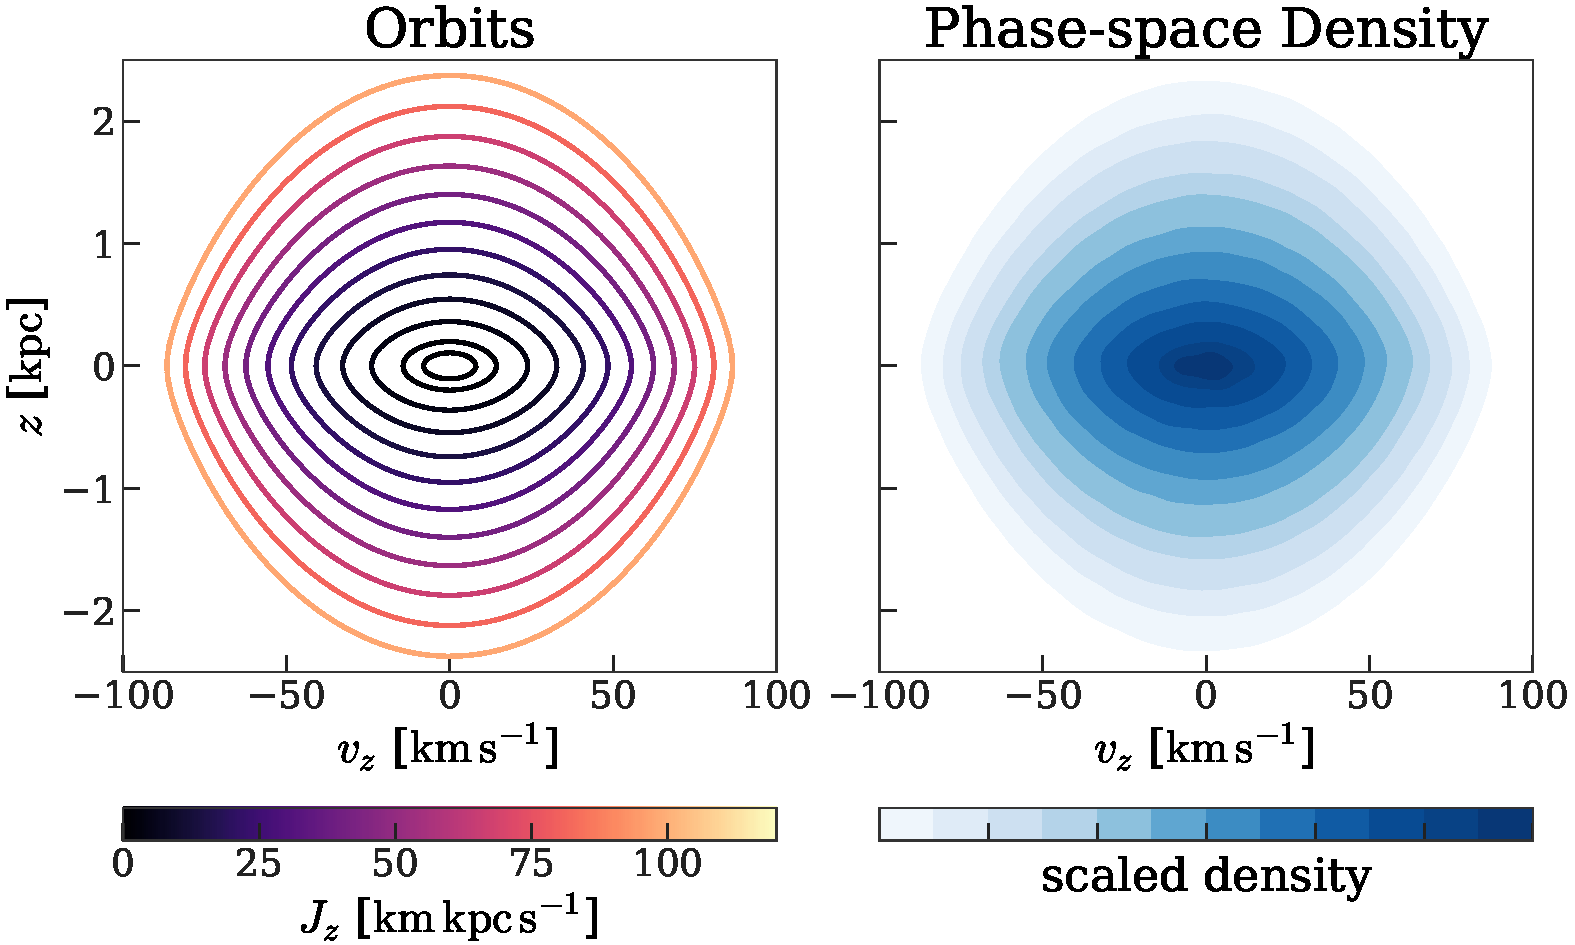
\includegraphics[width=\textwidth]{illustrate-zvz.pdf}
\end{center}
\caption{%
TODO
\label{fig:zvz}
}
\end{figure*}

Given a closed orbital trajectory in a 1D phase-space, we can estimate dynamical
quantities like the orbital actions, angles, and frequencies.
For example, in terms of the vertical position and velocity $z, v_z$, where an orbit can
be parametrized as $v_z(z)$, the vertical action $J_z$ and period $T_z$ are given by
\begin{align}
    J_z &= \frac{2}{\pi} \, \int_0^{z_{\textrm{max}}} \dd z \, v_z(z) \\
    T_z &= 4 \, \int_0^{z_{\textrm{max}}} \frac{\dd z}{v_z(z)}\quad ,
\end{align}
which can then be used to compute the vertical (angular) frequency $\Omega_z =
\frac{2\pi}{T_z}$.
For a given stellar position and velocity $z, v_z$ along an orbit, the vertical angle
$\theta_z$ can be computed as the fraction of an orbital period traversed up to that
point,
\begin{equation}
    \theta_z = \frac{2\pi}{T_z} \, \int_0^{z} \frac{\dd w}{v_z(w)} \quad ,
\end{equation}
where $w$ is an integration variable.
In principle, with infinite particle resolution, one could extract contours of constant
density (or stellar labels) from an observed phase-space distribution and numerically
estimate the integrals above.
In practice, however, this would be noisy and unstable in regions of low phase-space
density, which are often the most interesting (e.g., the transition from disk-dominated
to halo-dominated kinematics).
Instead, in what follows we outline a method for modeling the continuous phase-space
density that enables computing the dynamical quantities.


\subsection{Estimating Dynamical Quantities from the Phase-space Density}

Given a distribution of $N$ stellar positions and velocities $\{z, v_z\}_N$, our task is
to infer the parameters of a functional model for the number density $n(z, v_z)$ that
also allows use to compute the dynamical quantities ($J_z$, $\Omega_z$, $\theta_z$) for
any individual $z, v_z$.
With our assumption that the \df\ is phase-mixed, the number density should only depend
on the phase-space coordinates through the action, so that $n(z, v_z) = n(J_z(z, v_z))$
At fixed $z$, say $z=0$, we expect that $J_z$ increases with increasing $v_z$ (orbits
with larger velocity at the midplane will reach larger heights) and $\Omega_z$
decreases with increasing $v_z$ (orbits that reach larger heights above the midplane
have longer periods).
Similar arguments can be made at fixed $v_z=0$ in considering how $J_z$ and $\Omega_z$
vary with increasing $z$.
It is therefore useful to construct an ellipsoidal polar coordinate system in the $z,
v_z$ plane with a radius coordinate $r_z'$ and a corresponding angle coordinates
$\theta_z'$ defined as
\begin{align}
    r_z' &= \sqrt{z^2 \, \omega_0 + v_z^2 \, \omega_0^{-1}} \label{eq:rzp} \\
    \theta_z' &= \tan^{-1}\left(\frac{z}{v_z}\,\omega_0\right) \label{eq:thetazp}
\end{align}
where $\omega_0$ is a scale frequency.
The vertical action $J_z$ and frequency $\Omega_z$ should be close to monotonic
functions of this polar radius $r_z'$.

For example, in a simple harmonic oscillator (SHO) potential,
\begin{equation}
    \Phi(z) = \frac{1}{2} \, \omega^2 \, z^2
\end{equation}
the Hamiltonian (total energy per unit mass) is
\begin{equation}
    H(z, v_z) = E_z = \frac{1}{2} \, v_z^2 + \frac{1}{2} \, \omega^2 \,z^2
\end{equation}
and the orbital action $J_z$ is given by
\begin{equation}
    J_z = \frac{E_z}{\omega} \quad .
\end{equation}
All orbits have the same frequency $\omega$ and are elliptical in the 1D phase-space.
In this case, the scale frequency $\omega_0$ in $r_z'$ corresponds to the frequency of
the oscillator $\omega_0=\omega$, the radius $r_z'$ is related to the action $J_z$ as
\begin{equation}
    J_z = \frac{1}{2} r_z'^2
\end{equation}
and the conjugate angle $\theta_z$ (conjugate to the action $J_z$) is equal to the
ellipsoidal angle $\theta_z = \theta_z'$.
The phase-mixed \df\ $f(J_z)$ can therefore be expressed as some
function of the polar radius alone $f(J_z)=g(r_z')$.

Orbits in even simple galactic mass models are more complex.
For example, in a two-component mass model consisting of a Galactic disk embedded in a
dark matter halo, the morphology of an orbit will depend on whether it is confined to
the disk or whether it feels the transition from the disk- to the halo-dominated region
of the mass distribution.
Figure~\ref{fig:zvz} (left panel) is an illustration that shows several sample orbits
with different values of the vertical action (spaced uniformly in $\sqrt{J_z}$), all
with $J_R=0$ and the same $J_\phi$ in a two-component galaxy model consisting of a
Miyamoyo--Nagai disk component \citep{Miyamoto:1975} and a Navarro--Frenk--White (NFW)
halo component \citep{NFW:1996}.
For this toy galaxy model, parameters are chosen to roughly match the local circular
velocity and scale height of the Milky Way disk, but this potential model is only used
for illustrative purposes (the parameter values are not important).
For smaller values of the vertical action, orbits are close to elliptical in shape.
Moving out in ``radius'' or vertical action $J_z$, orbits have frequencies that decrease
with increasing action (which manifests as a changing axis ratio of the orbits).
For orbits with larger vertical action (i.e. orbits that reach scale heights more than a
few times the adopted scale height $h_z=0.25~\kpc$), the orbits begin to significantly
feel the influence of the dark matter halo and the orbital trajectory shapes become more
``pinched'' or ``diamond''-like near $z=0$.
We expect these features to be generic for slices of the vertical kinematics in galaxies
like the Milky Way: The vertical frequency should be a smooth function of the vertical
action, and orbits will have more complex morphologies (i.e. more complex than
ellipses).

Whereas in a SHO potential the orbital trajectories are functionally equivalent
(ellipses) and scaled by the value of the action, in a more generic galactic mass model
we expect the trajectories to distort away from ellipses.
As we saw in Figure~\ref{fig:zvz}, this distortion changes the orbital frequency of
orbits with increased size or vertical action (i.e., changes the scale frequency of the
ellipse), but also introduces a morphological change by making the orbits more
diamond-shaped, especially close to $z=0$.
In terms of action--angle coordinates, this means that the ellipsoidal angle introduced
above (Equation~\ref{eq:thetazp}) is no longer equal to the conjugate angle $\theta_z$,
and any functional model for the phase-mixed \df\ $f(J)$ must be a function of both the
ellipsoidal radius and angle:
\begin{equation}
    f(J) = g(r_z', \theta_z') \quad .
\end{equation}
We choose to express this density model as a function of an auxiliary variable $r_z$
that is defined as a low-order Fourier expansion distortion to the ellipsoidal radius
$r_z'$:
\begin{align}
    r_z &= r_z' \, \left[1 + \sum_m \epsilon_m(r_z') \, \cos{\left(m\,\theta_z'\right)}\right] \label{eq:rz} \\
    n(z, v_z) &= n(r_z(r_z', \theta_z'))
\end{align}
where $n(\cdot)$ represents a density function and $\epsilon_m(r_z')$ represents a
distortion amplitude, whose magnitude is hopefully must smaller than one for all
relevant values of $r_z'$ --- that is, we assume that
\begin{equation}
    |\epsilon_m(r_z')| \ll 1 \,\, \forall r_z', m \quad .
\end{equation}

With this parametrization, the action and frequency are monotonic and smooth functions
of the distorted radius $r_z$: $J_z = J_z(r_z)$ and $\Omega_z = \Omega_z(r_z)$.
We can also now compute the dynamical quantities with integrals over the ellipsoidal
angle $\theta_z'$
\begin{align}
    J_z(r_z) &= \frac{2}{\pi} \, \int_0^{\pi/2} \dd \theta_z' \, v_z(\theta_z')
        \, \left|\frac{\dd z}{\dd \theta_z'}\right| \\
    T_z &= 4 \, \int_0^{\pi/2} \frac{\dd \theta_z'}{v_z(\theta_z')}
        \, \left|\frac{\dd z}{\dd \theta_z'}\right|
\end{align}
where
\begin{align}
    v_z(\theta_z') &= \sqrt{\omega_0} \, r_z'(r_z, \theta_z') \, \cos{(\theta_z')} \\
    z(\theta_z') &= \frac{1}{\sqrt{\omega_0}} \, r_z'(r_z, \theta_z') \, \sin{(\theta_z')}
\end{align}
and $r_z'(r_z, \theta_z')$ in general has to be found by numerical root-finding of
Equation~\ref{eq:rz}.


\subsection{Estimating Dynamical Quantities from Statistics of Stellar Labels}

TODO: same thing as previous subsection, but $F(r_z)$ instead of $n(r_z)$


\section{Results} \label{sec:results}

For our implementation used in this article, we adopt the following:
\begin{align}
    m &= \left\{2, 4\right\} \\
    e_2(r_z') &\geq 0 \,\,\forall r_z'\\
    e_4(r_z') &\leq 0 \,\,\forall r_z'
\end{align}
and we use linear splines to represent the functions $n(r_z)$, $e_2(r_z')$, and
$e_4(r_z')$.


\subsection{Demonstration with a Simple Equilibrium Model}
\label{sec:eq-model}

Set up an Agama model, show that we can recover the acceleration field.


\subsection{Tests with a Perturbed Disk}
\label{sec:diseq-disk}

\subsection{Application to Data from \gaia\ Data Release 3}

Fit the vertical acceleration in a slice around the sun, ignoring selection function.
Show residuals: Phase spiral-o-rama

\subsection{Empirical Actions and Frequencies}
\label{sec:gaiadr3}


\section{Discussion} \label{sec:discussion}

\subsection{Limitation that our acceleration can depend on $v_z$}


\section{Summary and Conclusions} \label{sec:conclusions}


\begin{acknowledgements}

It is a pleasure to thank ...

% Funding for the Sloan Digital Sky Survey IV has been provided by the Alfred P.
% Sloan Foundation, the U.S. Department of Energy Office of Science, and the
% Participating Institutions. SDSS-IV acknowledges support and resources from the
% Center for High-Performance Computing at the University of Utah. The SDSS web
% site is www.sdss.org.

% SDSS-IV is managed by the Astrophysical Research Consortium for the
% Participating Institutions of the SDSS Collaboration including the Brazilian
% Participation Group, the Carnegie Institution for Science, Carnegie Mellon
% University, the Chilean Participation Group, the French Participation Group,
% Harvard-Smithsonian Center for Astrophysics, Instituto de Astrof\'isica de
% Canarias, The Johns Hopkins University, Kavli Institute for the Physics and
% Mathematics of the Universe (IPMU) / University of Tokyo, Lawrence Berkeley
% National Laboratory, Leibniz Institut f\"ur Astrophysik Potsdam (AIP),
% Max-Planck-Institut f\"ur Astronomie (MPIA Heidelberg), Max-Planck-Institut
% f\"ur Astrophysik (MPA Garching), Max-Planck-Institut f\"ur Extraterrestrische
% Physik (MPE), National Astronomical Observatories of China, New Mexico State
% University, New York University, University of Notre Dame, Observat\'ario
% Nacional / MCTI, The Ohio State University, Pennsylvania State University,
% Shanghai Astronomical Observatory, United Kingdom Participation Group,
% Universidad Nacional Aut\'onoma de M\'exico, University of Arizona, University
% of Colorado Boulder, University of Oxford, University of Portsmouth, University
% of Utah, University of Virginia, University of Washington, University of
% Wisconsin, Vanderbilt University, and Yale University.

This work has made use of data from the European Space Agency (ESA) mission
{\it Gaia} (\url{https://www.cosmos.esa.int/gaia}), processed by the {\it Gaia}
Data Processing and Analysis Consortium (DPAC,
\url{https://www.cosmos.esa.int/web/gaia/dpac/consortium}). Funding for the DPAC
has been provided by national institutions, in particular the institutions
participating in the {\it Gaia} Multilateral Agreement.

\end{acknowledgements}

\software{
    Astropy \citep{astropy:2013, astropy:2018, astropy:2022},
    gala \citep{gala},
    IPython \citep{ipython},
    numpy \citep{numpy},
    % pymc3 \citep{Salvatier2016},
    % schwimmbad \citep{schwimmbad:2017},
    scipy \citep{scipy}.
}

\bibliographystyle{aasjournal}
\bibliography{empirical-af}

\end{document}
